\documentclass[helvetica,utf8,english,11pt]{europecv}
% >german< für deutsche Begriffe

\usepackage{graphicx,url}
\usepackage{ifthen,eso-pic}

\newboolean{privat}
\setboolean{privat}{false}

\usepackage[sfdefault]{plex-sans}
\usepackage{microtype}

\usepackage{csquotes}
\usepackage[a4paper,top=1.5cm,left=1cm,right=1.4cm,bottom=2.0cm]{geometry}

\newcommand{\until}{\,--\,}

\ecvname{Donald Duck}
\ecvaddress{Erpelweg 1, 12345 Entenhausen}
\ecvtelephone{0152-213458979}
\ecvfax{0152-2134589791}
\ecvemail{donald@duck.com}
\ecvnationality{World Citizen}

\AddToShipoutPicture*{%
	\put(410,700){%
		\fbox{%
			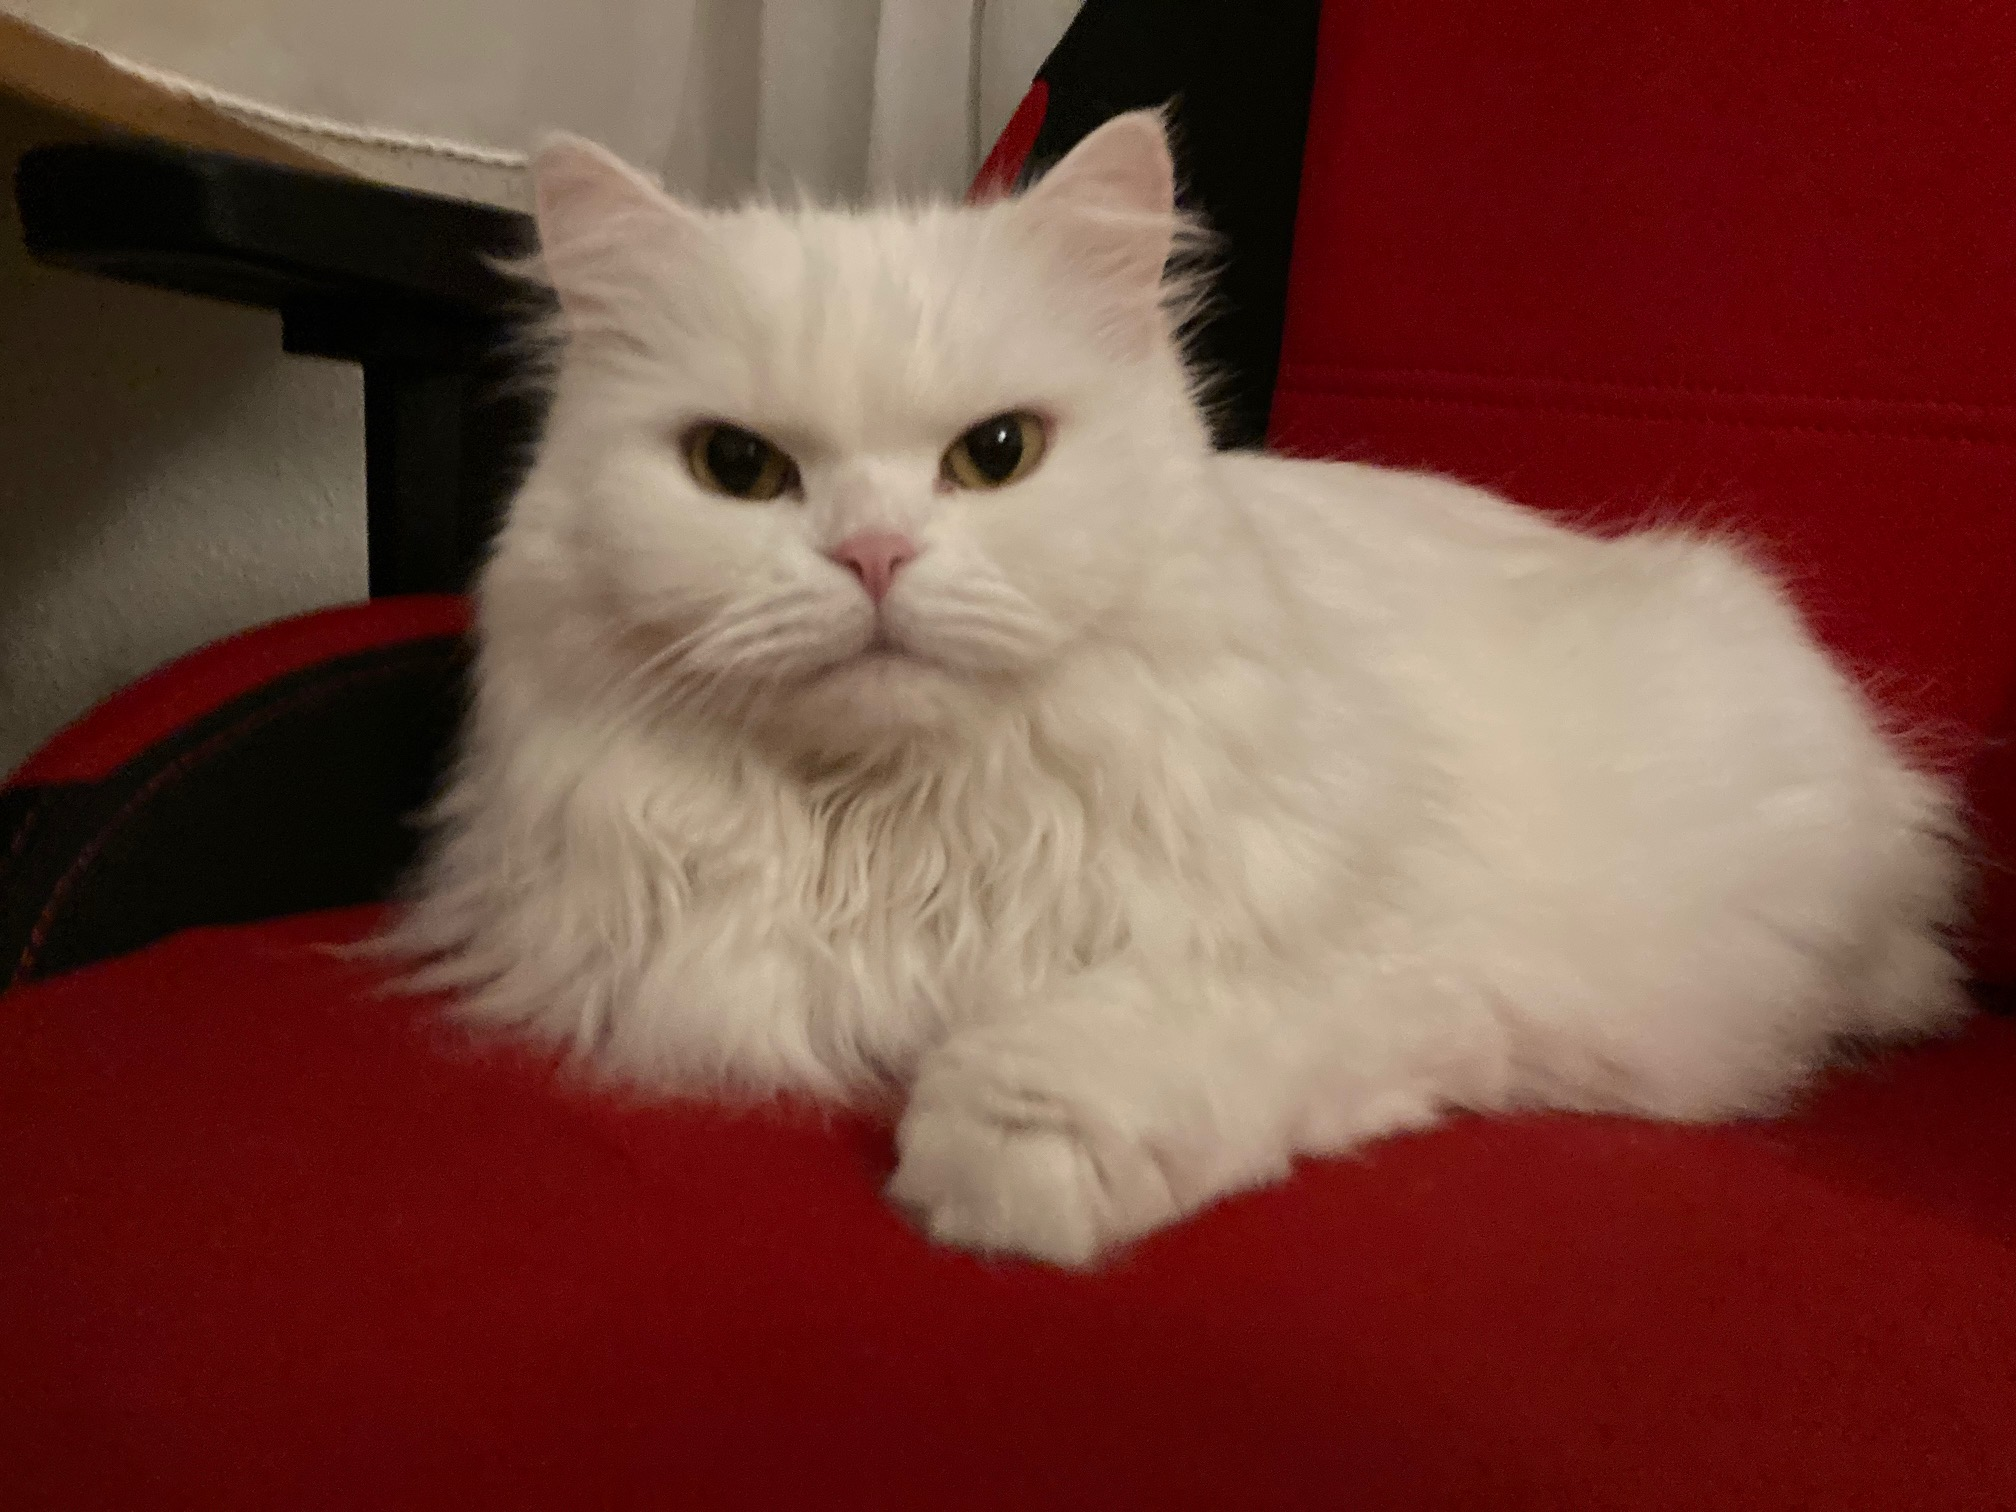
\includegraphics[height=3cm]{Katze2.jpg}
		}
	}
}

\begin{document}
\begin{europecv}
\ecvpersonalinfo

\ecvsection{Work experience}

\ecvitem{Dates (from--to)}{\textbf{1/2020\until present}}
\ecvitem{Name of employer}{Duck Enterprises}
\ecvitem{Type of business or sector}{Banking}
\ecvitem{Main activities and responsibilities}{Assistant of CEO}

\ecvitem{}{}
\ecvitem{Dates (from--to)}{\textbf{1/2015\until 12/2019}}
\ecvitem{Name of employer}{Entenhause Real Estate}
\ecvitem{Type of business or sector}{Real Estate}
\ecvitem{Main activities and responsibilities}{Facility Manager}

\ecvsection{Education and Training}

\ifthenelse{\boolean{privat}}{%
	\ecvitem{Dates (from--to)}{\textbf{2005\until 2015}}
	\ecvitem{Place}{Entenhausen Gesamtschule}
	\ecvitem{Title of Qualification awarded}{Fachabitur}
	\ecvitem{Main subjects}{Physics and Mathematics}
}{%
% Private Daten nicht mit ausgeben
}

\ecvsection{Personal skills and competences}

\ecvitem{\large\textsc{Other languages}}{}

\ecvitem{}{\textbf{English}}
\ecvitem{Reading Skills}{Excellent}
\ecvitem{Writing skills}{Excellent}
\ecvitem{Verbal skills}{Excellent}

\ecvitem{}{\textbf{Spanish}}
\ecvitem{Reading skills}{Basic}
\ecvitem{Writing skills}{Basic}
\ecvitem{Verbal skills}{Basic}

\end{europecv}
\end{document}


